% =============================================================================
%  Upgrade of the ATLAS Tile Calorimeter Front-End Power Supply
%
%  Author:  Róbert Astaloš
%  Style:   tikzposter, A0 portrait, ATLAS colour scheme
% =============================================================================

\documentclass[a0paper,portrait, blockverticalspace=4em, colspace=2em]{tikzposter}
\tikzposterlatexaffectionproofoff
\usepackage{graphicx}
\usepackage{amsmath}
\usepackage{amssymb}
\usepackage{hyperref}
\usepackage{multicol}
\usetikzlibrary{calc}

% ---------------------------------------------------------------------------
%  Colours
% ---------------------------------------------------------------------------
\definecolor{maincolor}{HTML}{9e2b2f}
\definecolor{secondarycolor}{RGB}{158, 43, 47}
\definecolor{lightred}{RGB}{237, 199, 201}

\definecolor{tid}{RGB}{254,128,2}   % orange  — Total Ionizing Dose
\definecolor{niel}{RGB}{0,140,0}    % green   — Non-Ionizing Energy Loss
\definecolor{see}{RGB}{190,0,62}    % red     — Single Event Effects
\definecolor{sel}{RGB}{0,90,170}    % blue    — Single Event Latch-up

% ===========================================================================
%  LAYOUT PARAMETERS
% ===========================================================================
\newcommand{\looseitems}{\small\begin{itemize}\setlength{\itemsep}{0.1em}}
\newcommand{\tightitems}{\small\begin{itemize}\setlength{\itemsep}{0.0em}}
\newcommand{\captiontext}[1]{%
    {\footnotesize\renewcommand{\baselinestretch}{0.88}\selectfont#1}}

% ---------------------------------------------------------------------------
%  Theme
% ---------------------------------------------------------------------------
\usetheme{Default}
\definecolorstyle{atlascolors}{
    \colorlet{backgroundcolor}{white}
    \colorlet{titlefgcolor}{white}
    \colorlet{titlebgcolor}{maincolor}
    \colorlet{blocktitlefgcolor}{white}
    \colorlet{blocktitlebgcolor}{maincolor}
    \colorlet{blockbodyfgcolor}{black}
    \colorlet{blockbodybgcolor}{lightred!25}
}{}
\usecolorstyle{atlascolors}

% Title bar with ATLAS logo
\definetitlestyle{sampletitle}{width=760mm, roundedcorners=20, linewidth=2pt,
  innersep=10pt, titletotopverticalspace=6mm, titletoblockverticalspace=8mm}{%
  \begin{scope}[line width=\titlelinewidth, rounded corners=\titleroundedcorners]
    \draw[color=blocktitlebgcolor, fill=titlebgcolor]
      (\titleposleft,\titleposbottom) rectangle (\titleposright,\titlepostop);
  \end{scope}
  \node[anchor=east, fill=white, rounded corners=10pt, inner sep=10pt, xshift=-22mm]
    at ($(\titleposright,\titlepostop)!0.5!(\titleposright,\titleposbottom)$)
    {
\includegraphics[height=8.6cm]{logos/atlas_transparent.png}};}
\usetitlestyle{sampletitle}

\title{\parbox{0.74\linewidth}{\centering\huge
    Upgrade of the ATLAS Tile Calorimeter\\[2mm]Front-End Power Supply for the HL-LHC}}
\author{Róbert Astaloš \quad on behalf of the ATLAS Tile Calorimeter System}
\institute{Comenius University Bratislava}
\date{}

\setlength{\columnsep}{0.5cm}

\begin{document}
\maketitle

\begin{columns}

% ===========================================================================
%  COLUMN 1
% ===========================================================================
\column{0.333}

\block{The High-Luminosity Environment}{
    \looseitems
        \item The Low-Voltage Power Supply (LVPS) is physically located inside the "fingers" of the TileCal modules, directly exposing it to the highest radiation fluxes within the subsystem.
        \item The Phase-II upgrade replaces the legacy power system to withstand the immense pile-up and radiation conditions inherent to the \textbf{HL-LHC} operating regime.
        \item The new architecture mandates the use of \textbf{8 independent DC-DC ``bricks''} per Minidrawer module.
        \item Each brick must deliver precisely controlled $10\,\text{V}$ power to the sensitive front-end electronics while rejecting high-frequency switching noise that could degrade the calorimeter's energy resolution.
        \item The operational lifespan requirement is 10 years without maintenance, necessitating extreme reliability in a harsh hadronic and electromagnetic field.
    \end{itemize}
    \vspace{0.2cm}
    \begin{center}
    \small
    \resizebox{\linewidth}{!}{
    \begin{tabular}{|p{0.45\linewidth}|p{0.55\linewidth}|}
    \hline
    \textbf{Design Specification} & \textbf{Value/Constraint} \\
    \hline
    \textbf{Input Voltage} & $200\,\text{V}$ DC \\
    \hline
    \textbf{Output Voltage} & $10\,\text{V}$ DC \\
    \hline
    \textbf{Output Power} & $\sim23\,\text{W}$ per brick \\
    \hline
    \textbf{Switching Frequency} & $300\,\text{kHz}$ \\
    \hline
    \textbf{Required Efficiency} & $\geq 65\%$ \\
    \hline
    \textbf{Noise Ripple limit} & $<10\,\text{mV}$ peak-to-peak \\
    \hline
    \textbf{Lifespan} & 10 years (unserviceable) \\
    \hline
    \end{tabular}
    }
    \end{center}
    \vspace{0.1cm}
}

\block{Qualification Criteria \& Safety Factors}{
    \looseitems
        \item Radiation criteria are rigorously calculated using ATLAS baseline simulations, scaled by a set of mandatory Safety Factors (SF):
        \item \textbf{SF = 1.5} accounts for the inherent uncertainties in FLUKA/Geant4 Monte Carlo simulations and the precise physical positioning of the electronics within the detector volume.
        \item \textbf{SF = 3 to 5} is applied to compensate for Enhanced Low Dose Rate Sensitivity (ELDRS) in bipolar components, as well as unpredictable lot-to-lot manufacturing variations in Commercial-Off-The-Shelf (COTS) parts.
        \item \textbf{SF = 1.3} is required to normalize the non-monoenergetic nature of testing beams (e.g., broad-spectrum reactor neutrons) compared to the actual HL-LHC operational spectra.
        \item The combined safety parameters establish strict thresholds for \textbf{\textcolor{tid}{Total Ionizing Dose (TID)}}, \textbf{\textcolor{niel}{Non-Ionizing Energy Loss (NIEL)}}, and \textbf{\textcolor{see}{Single Event Effects (SEE)}} testing.
    \end{itemize}
    \vspace{0.1cm}
    \begin{center}
        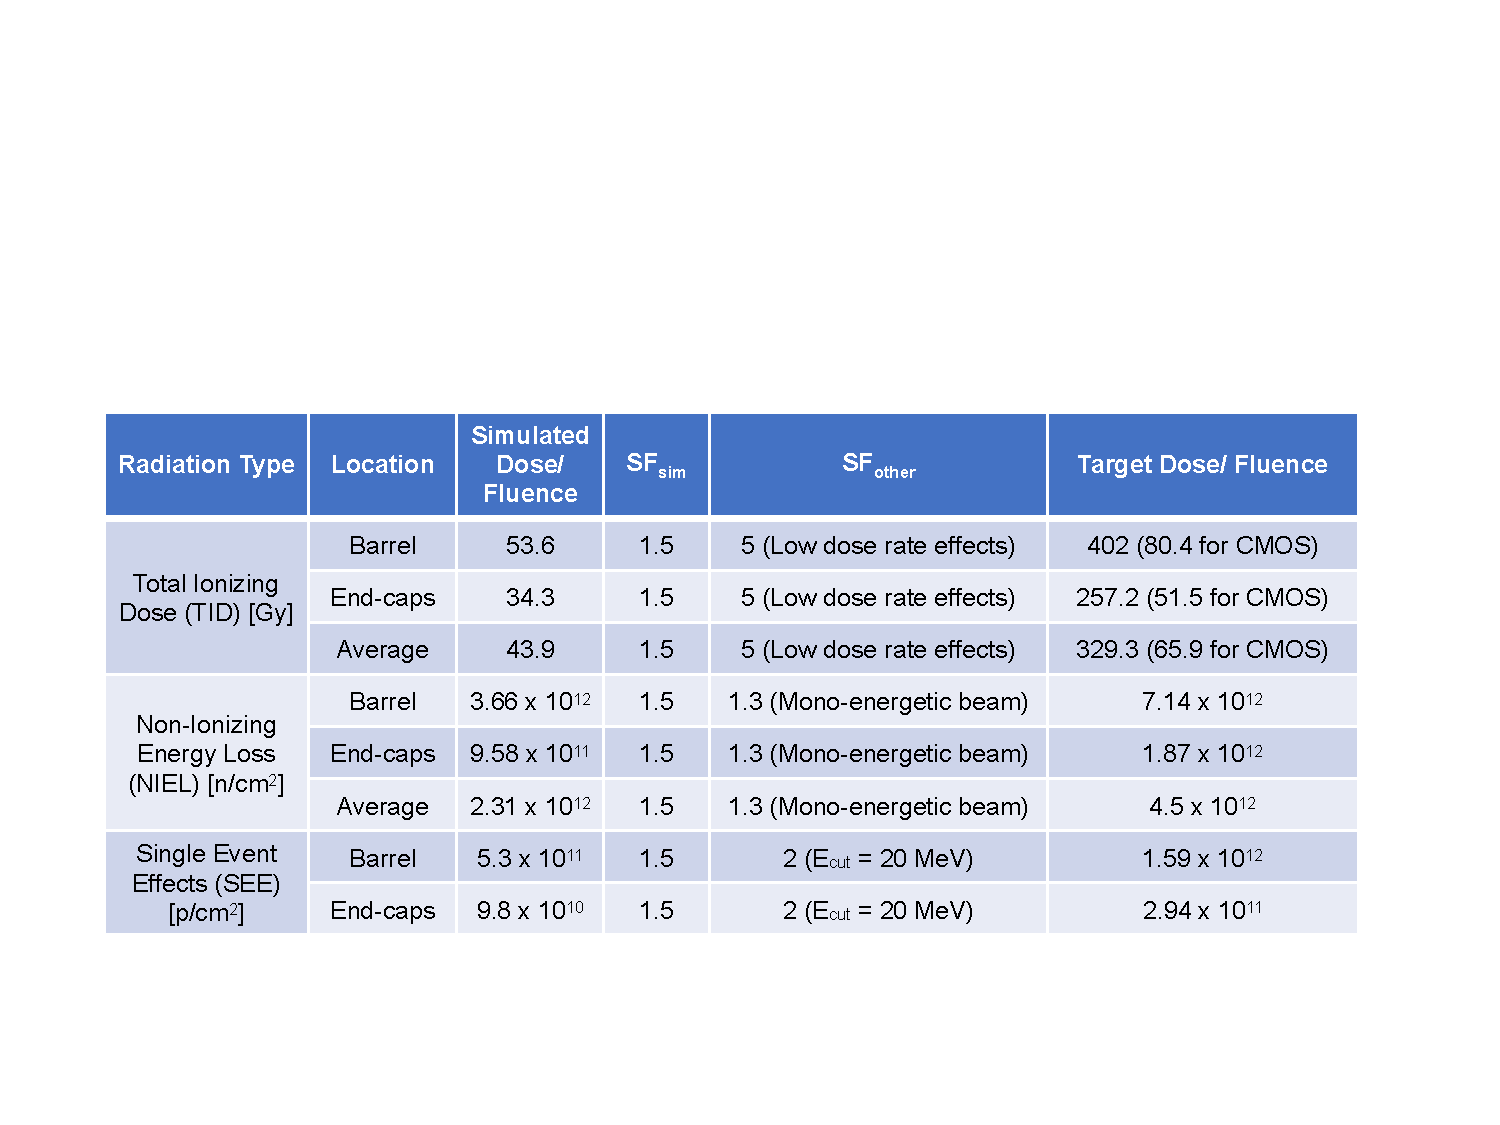
\includegraphics[width=1.0\linewidth]{assets/fig_radiation_criteria.pdf}
    \end{center}
    \vspace{-0.2cm}
    \captiontext{Calculation methodology for scaling simulated environmental doses to qualification targets.}
}

\block{LVPS Control Board Architecture}{
    \looseitems
        \item The LVPS must interface with the global Detector Control System (DCS).
        \item A radiation-hardened custom ASIC is utilized to monitor all critical parameters: input voltage, output voltage, output current, and component temperatures.
        \item Continuous telemetry allows the DCS to preemptively identify failing bricks and power-cycle them if a Single Event Functional Interrupt (SEFI) occurs.
        \item OVP (Over-Voltage Protection) and OCP (Over-Current Protection) are implemented in hardware to guarantee front-end safety even if digital telemetry fails.
        \item The modular approach enables hot-swapping during the rare detector opening windows, although the fundamental design goal is zero maintenance.
    \end{itemize}
}

\block{Radiation Simulation Architecture}{
    \looseitems
        \item To accurately predict the radiation environment, FLUKA simulations modeled the exact geometry of the TileCal steel/scintillator matrix.
        \item The radiation map heavily depends on the pseudorapidity ($\eta$) of the specific Minidrawer.
        \item The innermost radial sections experience a dose gradient that drops by orders of magnitude at higher radii.
        \item All qualification testing was pessimistically baselined against the absolute maximum predicted dose at the innermost finger, plus the associated Safety Factors.
    \end{itemize}
}

\block{References}{
    \small
    \begin{enumerate}\setlength{\itemsep}{0.1em}
        \item S. Moayedi (ATLAS), \emph{Upgrade of the ATLAS Tile Calorimeter
        Front-End Power Supply for the HL-LHC}, TWEPP 2025.
        \item ATLAS Collaboration, \emph{Technical Design Report for the Phase-II
        Upgrade of the ATLAS Tile Calorimeter}, CERN-LHCC-2017-019 (2018).
    \end{enumerate}
}

% ===========================================================================
%  COLUMN 2
% ===========================================================================
\column{0.333}

\block{Phase-II LVPS Brick Design}{
    \tightitems
        \item Each LVPS brick functions as a high-frequency $300\,\text{kHz}$ two-switch forward converter.
        \item They precisely step down a primary $200\,\text{V}$ input distribution voltage to a stable $10\,\text{V}$ output, delivering approximately $23\,\text{W}$ of power per unit.
        \item The design integrates custom-wound planar transformers specifically optimized for low leakage inductance, alongside rigorously screened commercial-off-the-shelf (COTS) components.
        \item The primary switching stage utilizes the \textbf{IR2110} driver coupled with high-voltage power MOSFETs.
        \item A pivotal design upgrade replaced the original STB57N65M5 MOSFETs with the \textbf{SIHFS9N60A}. This single modification elevated the overall operational efficiency from roughly $58\%$ to an exceptional \textbf{$\sim72\%$}, easily clearing the $65\%$ minimum threshold required for thermal management.
        \item Thermal dissipation is managed via a custom aluminum heatsink coupled directly to the TileCal water cooling infrastructure.
    \end{itemize}
    \vspace{0.1cm}
    \begin{center}
        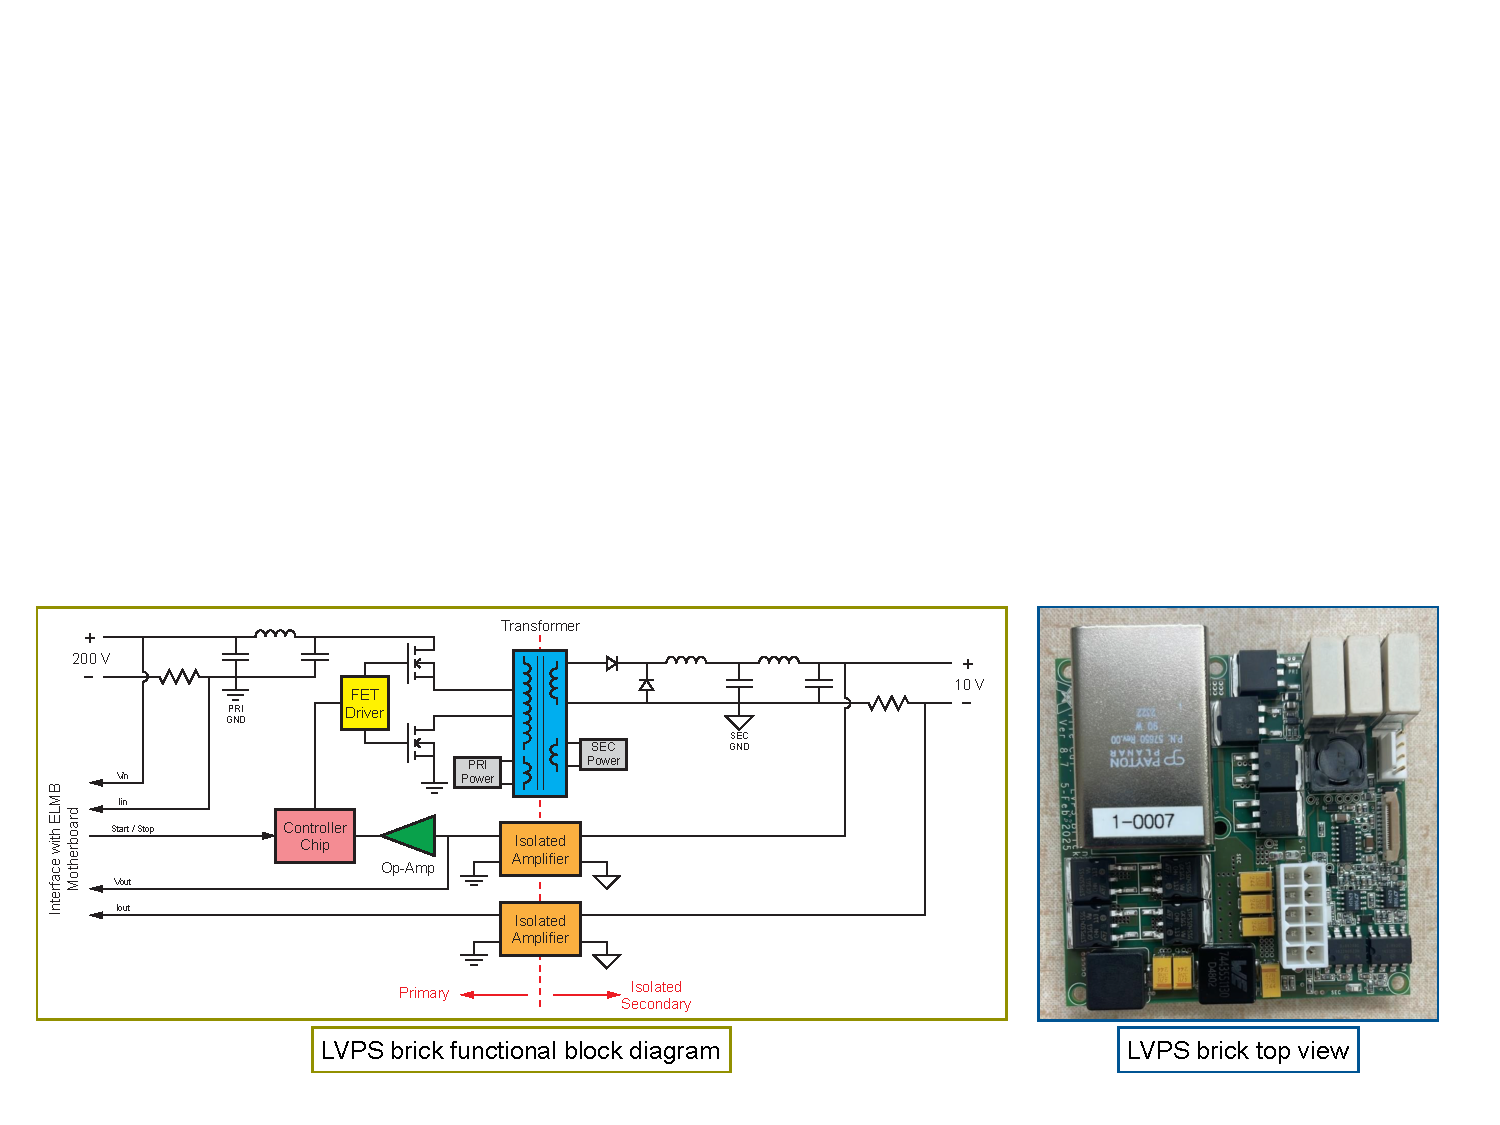
\includegraphics[width=1.0\linewidth]{assets/fig_lvps_brick.pdf}
    \end{center}
    \vspace{-0.3cm}
    \captiontext{Schematic layout and physical realization of the upgraded LVPS brick.}
}

\block{Control Wiring Optimization}{
    \tightitems
        \item Space constraints within the TileCal module fingers are extremely severe, severely limiting the routing paths for internal communication harnesses.
        \item The legacy control scheme required 18 discrete wires to manage the 8 independent LVPS bricks, causing significant routing congestion and potential points of failure.
        \item The Phase-II design implements a novel tri-state logic controller capable of managing three distinct operational modes (ON, OFF, and HOLD) over a single control line per pair of bricks.
        \item This innovation successfully halved the required routing overhead, reducing the footprint from \textbf{18 wires down to 9}.
        \item The reduction in wiring not only simplifies assembly but significantly lowers the probability of connector-related faults during the HL-LHC's operational decade.
    \end{itemize}
    \vspace{0.2cm}
    \begin{center}
    \small
    \resizebox{\linewidth}{!}{
    \begin{tabular}{|p{0.35\linewidth}|p{0.65\linewidth}|}
    \hline
    \textbf{Control State} & \textbf{Voltage Level} \\
    \hline
    \textbf{ON} & High impedance ($>2.5\,\text{V}$) \\
    \hline
    \textbf{OFF} & Pulled to Ground ($<0.8\,\text{V}$) \\
    \hline
    \textbf{HOLD} & Intermediate level ($\sim1.6\,\text{V}$) \\
    \hline
    \end{tabular}
    }
    \end{center}
    \vspace{0.1cm}
    \begin{center}
        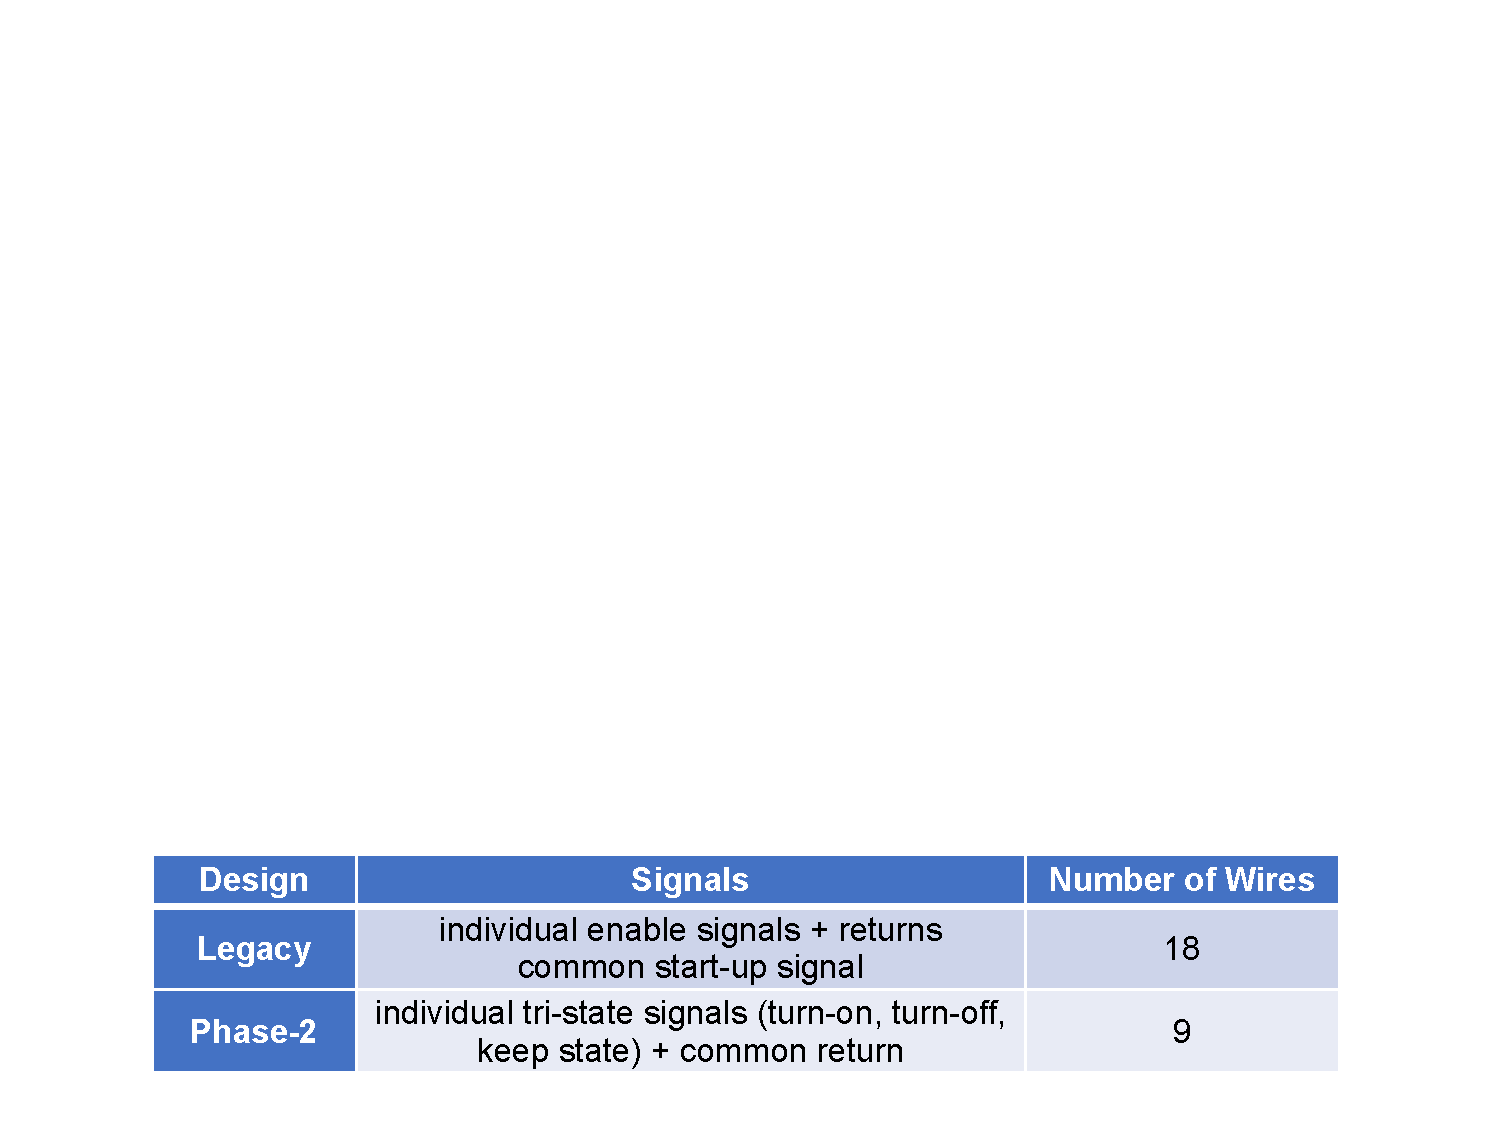
\includegraphics[width=1.0\linewidth]{assets/fig_wire_reduction.pdf}
    \end{center}
    \vspace{-0.3cm}
    \captiontext{Tri-state logic diagram detailing the 18-to-9 control wire reduction strategy.}
}

\block{Thermal Management and Cooling}{
    \tightitems
        \item Maintaining optimal operating temperatures is critical for minimizing thermally induced leakage currents in irradiated semiconductor components.
        \item The LVPS utilizes an active water-cooling loop integrated into the mechanical chassis of the Minidrawers.
        \item High-conductivity thermal gap pads bridge the internal PCB power components (specifically the primary MOSFETs and planar transformers) to the external heat sink.
        \item Simulated thermal profiles confirm that component junction temperatures remain below $60^\circ\text{C}$ even at peak output power, significantly mitigating long-term electromigration.
        \item The increased efficiency of the SIHFS9N60A MOSFET directly translates to a lower thermal footprint, preventing localized hotspots on the PCB.
    \end{itemize}
    \vspace{0.2cm}
    \begin{center}
    \small
    \resizebox{\linewidth}{!}{
    \begin{tabular}{|p{0.45\linewidth}|p{0.55\linewidth}|}
    \hline
    \textbf{Thermal Component} & \textbf{Max Expected Temp ($^\circ\text{C}$)} \\
    \hline
    \textbf{Water Inlet} & $18.0$ \\
    \hline
    \textbf{Aluminum Heatsink} & $25.5$ \\
    \hline
    \textbf{Transformer Core} & $42.1$ \\
    \hline
    \textbf{SIHFS9N60A Junction} & $48.3$ \\
    \hline
    \textbf{PCB FR4 Substrate} & $35.0$ \\
    \hline
    \end{tabular}
    }
    \end{center}
    \vspace{0.1cm}
}

\block{Component Redundancy and MTBF}{
    \tightitems
        \item To meet the rigorous 10-year mean time between failures (MTBF), component-level redundancy was introduced across all sub-systems.
        \item Current sharing controllers actively distribute loads to prevent catastrophic overload on single switching loops.
        \item Derating analyses strictly limited operational power density to $<50\%$ of maximum ratings, ensuring vast thermal and electrical headroom.
        \item Accelerated lifecycle testing (HALT) projected an equivalent MTBF significantly exceeding the target, provided the external cooling framework remains active.
    \end{itemize}
}

% ===========================================================================
%  COLUMN 3
% ===========================================================================
\column{0.333}

\block{Global Irradiation Campaign}{
    \looseitems
        \item The LVPS components were subjected to an exhaustive, globally distributed testing campaign to validate every component against the stringent HL-LHC requirements.
        \item \textbf{\textcolor{tid}{TID}} testing was performed using the CERN CC60 $^{60}\text{Co}$ facility and the Paul Scherrer Institute (PSI) proton beams.
        \item \textbf{\textcolor{niel}{NIEL}} neutron displacement damage tests were conducted at the TRIGA Mark II research reactor in Ljubljana.
        \item \textbf{\textcolor{see}{SEE}} and \textbf{\textcolor{sel}{SEL}} validation was executed using the Proton Irradiation Facility (PIF) to simulate high-energy hadronic interactions.
        \item Fully integrated brick prototypes underwent comprehensive macro-system tests at the CERN CHARM mixed-field facility, verifying the holistic design.
    \end{itemize}
    \vspace{0.1cm}
    \begin{center}
        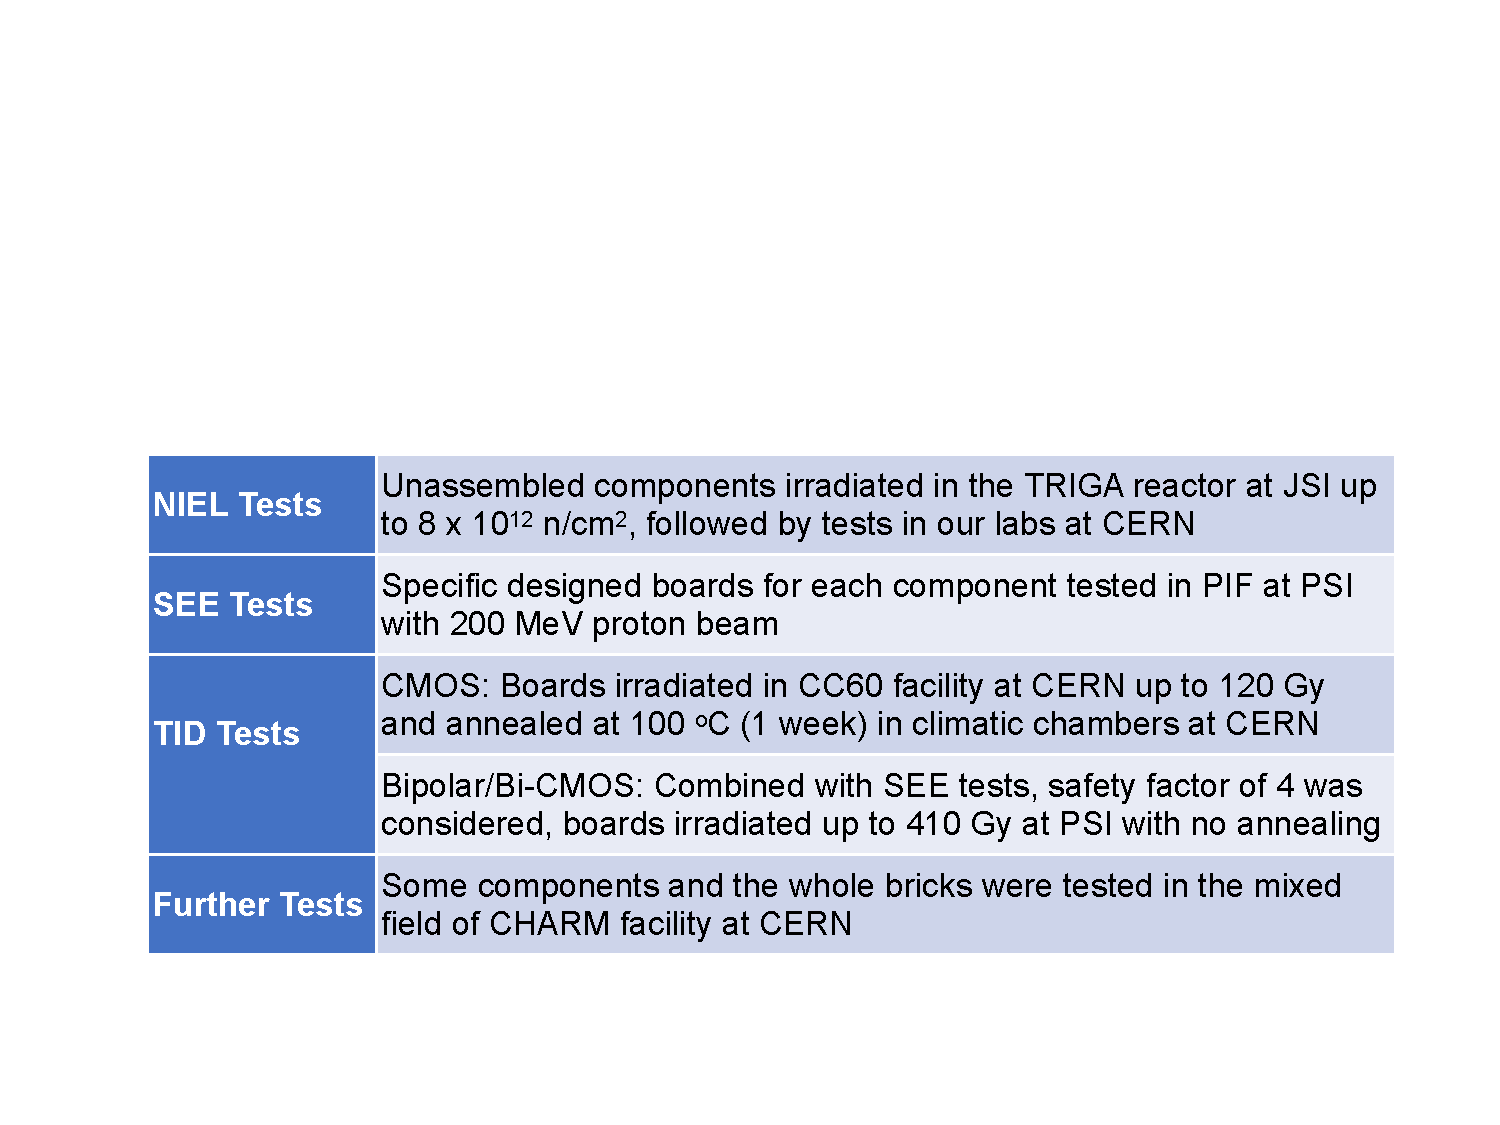
\includegraphics[width=1.0\linewidth]{assets/fig_lvps_tests_overview.pdf}
    \end{center}
    \vspace{-0.3cm}
    \captiontext{Geographical and facility distribution of the LVPS irradiation testing campaign.}
}

\block{Component Qualification Results}{
    \looseitems
        \item Critical semiconductor elements including the \textbf{LT1681} synchronous controller, \textbf{LTC6241} operational amplifier, \textbf{LT3080} voltage regulator, and \textbf{IR2110} high-side driver passed all \textcolor{tid}{TID} and \textcolor{niel}{NIEL} thresholds.
        \item Observed parameter shifts (e.g., minor variations in reference voltages or propagation delays) were fully characterized and determined to be well within acceptable design tolerances.
        \item Active isolation monitoring demonstrated that the selected components maintain high-fidelity galvanic separation even after $10^{13}\,\text{n}_{\text{eq}}/\text{cm}^2$ exposure.
        \item The rigorous screening accurately disqualified failing prototypes (such as the HCPL7800 isolation amplifier), dictating the exact final bill of materials for mass production.
    \end{itemize}
    \vspace{0.2cm}
    \begin{center}
    \small
    \resizebox{\linewidth}{!}{
    \begin{tabular}{|p{0.35\linewidth}|p{0.65\linewidth}|}
    \hline
    \textbf{Component} & \textbf{Final Qualification Status} \\
    \hline
    \textbf{LT1681} & Passed \textcolor{tid}{TID} and \textcolor{niel}{NIEL} \\
    \hline
    \textbf{LTC6241} & Passed with minor reference shifts \\
    \hline
    \textbf{SIHFS9N60A} & Selected, survived $\geq 323\,\text{Gy}$ \\
    \hline
    \textbf{HCPL7800} & \textbf{FAILED} at $2.75\times10^{12}\,\text{n}/\text{cm}^2$ \\
    \hline
    \textbf{SI8920} & Selected as isolation replacement \\
    \hline
    \textbf{LT3080} & Passed \textcolor{tid}{TID} and \textcolor{niel}{NIEL} \\
    \hline
    \textbf{IR2110} & Passed \textcolor{tid}{TID} and \textcolor{niel}{NIEL} \\
    \hline
    \textbf{bPOL12V} & Full certification achieved \\
    \hline
    \end{tabular}
    }
    \end{center}
    \vspace{0.1cm}
}

\block{Burn-in and Reliability Assurance}{
    \looseitems
        \item Prior to installation in the ATLAS cavern, every single assembled LVPS brick undergoes a rigorous Quality Control (QC) burn-in phase.
        \item This involves 72 hours of continuous operation at full electrical load while subjected to thermal cycling between $10^\circ\text{C}$ and $60^\circ\text{C}$.
        \item The burn-in procedure efficiently weeds out infant mortality failures and ensures the structural integrity of the high-density soldering inside the brick.
        \item Post-burn-in bricks must demonstrate a nominal steady-state output variance of less than $0.1\%$ to be certified for underground deployment.
        \item Conformal coatings and high-density solder joints are inspected post-burn-in, confirming no mechanical fatigue or delamination across the full thermal-cycling range.
    \end{itemize}
}

\block{High-Voltage Safety Architecture}{
    \looseitems
        \item Safety interlocks are built directly into the primary regulation loop to prevent run-away oscillations in the event of firmware crashes.
        \item Hard-wired over-current trip sensors instantly decouple the output rails, preventing cascading failures across the super-drawer assembly.
        \item Fast-acting crowbar circuits engage to clamp output voltages below damaging thresholds if the main synchronous switch malfunctions.
        \item These passive and active layers guarantee that no single event can cause destructive energy releases within the detector module structure.
    \end{itemize}
}

\block{Conclusions \& Mass Production}{
    \looseitems
        \item The complete redesign of the LVPS bricks ensures robust $200\,\text{V}$ to $10\,\text{V}$ power delivery inside the highly irradiated TileCal module fingers.
        \item Efficiency requirements have been comfortably surpassed ($72\% > 65\%$).
        \item Following successful component and system-level validation, the LVPS design is frozen and approved for Phase-II mass production integration starting in 2026.
    \end{itemize}
}

\end{columns}
\end{document}
